\documentclass[9pt]{beamer}

% Choose a professional theme
\usetheme{CambridgeUS} % Alternative themes: Boadilla, Singapore, etc.

% Choose a color theme (optional)
\usecolortheme{seahorse} % You can explore other color themes like 'beaver', 'dolphin', etc.

% Packages
\usepackage{amsmath}
\usepackage{graphicx}
\usepackage{booktabs}

% Title information
\title[CVAE Implementation]{Analysis of CVAE Implementation}
\subtitle{Enhancing Performance through Loss Function Optimization and Architecture Tuning}

% Author and Supervisor
\author{A.Ghanaatian\and Supervisor: Prof. Caragea}

% Date
\date{\today} % You can replace \today with a specific date if preferred

\begin{document}

\begin{frame}
  \titlepage
\end{frame}

% Slide 2
\begin{frame}{Introduction}
  \begin{itemize}
    \item \textbf{Objective}: Improve the model by implementing several key enhancements:
    \begin{itemize}
      \item Added plotting to compare real vs. predicted values.
      \item Incorporated an \textbf{Energy Loss}$^2$ component to minimize energy discrepancies.
      \item Included \textbf{MRE}$^2$ in the loss function for differentiability and metric minimization.
      \item Fine-tune all Parameters and Hyper-Parameters to optimize the new loss function and training phase to get a better model
    \end{itemize}
  \end{itemize}
\end{frame}

% Slide 3
\begin{frame}{Understanding Energy Components}
  \begin{itemize}
    \item \textbf{Energy Calculations} are being used for the \textbf{Energy Loss} term in our loss function.
    \item Components involved:
    \begin{enumerate}
      \item \textbf{Kinetic Energy (KE)}
      \item \textbf{Potential Energy (PE)}
      \item \textbf{Error Calculation between KE and PE}
    \end{enumerate}
  \end{itemize}
\end{frame}

% Slide 4
\begin{frame}{Kinetic Energy (KE)}
  The total kinetic energy is the sum of the kinetic energies of Carbon (C), Oxygen (O), and Sulfur (S):
  \[
  KE = KE(C) + KE(O) + KE(S)
  \]
  Where:
  \[
  \begin{aligned}
  KE(C) &= \frac{p_{Cx}^2}{2m_C} + \frac{p_{Cy}^2}{2m_C} + \frac{p_{Cz}^2}{2m_C} \\
  KE(O) &= \frac{p_{Ox}^2}{2m_O} + \frac{p_{Oy}^2}{2m_O} + \frac{p_{Oz}^2}{2m_O} \\
  KE(S) &= \frac{p_{Sx}^2}{2m_S} + \frac{p_{Sy}^2}{2m_S} + \frac{p_{Sz}^2}{2m_S}
  \end{aligned}
  \]
  Masses:
  \[
  m_C = 21894.71361 \quad m_O = 29164.39289 \quad m_S = 58441.80487
  \]
\end{frame}

% Slide 5
\begin{frame}{Potential Energy (PE)}
  The potential energy is calculated based on the distances between the atoms:
  \[
  PE = \frac{4}{r_{CO}} + \frac{4}{r_{CS}} + \frac{4}{r_{OS}}
  \]
  Where:
  \[
  \begin{aligned}
  r_{CO} &= \sqrt{(c_x - o_x)^2 + (c_y - o_y)^2 + (c_z - o_z)^2} \\
  r_{CS} &= \sqrt{(c_x - s_x)^2 + (c_y - s_y)^2 + (c_z - s_z)^2} \\
  r_{OS} &= \sqrt{(o_x - s_x)^2 + (o_y - s_y)^2 + (o_z - s_z)^2}
  \end{aligned}
  \]
\end{frame}

% Slide 6
\begin{frame}{Energy Error Calculation}
  The error between kinetic and potential energy is calculated as:
  \[
  \text{Error} = \frac{\left| KE - PE \right|}{\left| KE \right|}
  \]
  \begin{itemize}
    \item This error is minimized in the \textbf{Energy Loss} component of our loss function.
  \end{itemize}
\end{frame}

% Slide 7: Split into two slides

% Original Slide 7: Comprehensive Loss Function
% Now split into Slide 7 and Slide 8

% Slide 7
\begin{frame}{Comprehensive Loss Function (Part 1)}
  The combined \textbf{Loss Function} can be expressed as:
  \[
  \text{Loss} = \alpha_1 \cdot \text{Energy Diff}^2 + \alpha_2 \cdot \text{MRE}^2 + \alpha_3 \cdot \text{MSE}
  \]
  Where:
  \begin{enumerate}
    \setcounter{enumi}{0} % Start from the second item
    \item \textbf{Energy Difference}:
      \[
      \text{Energy Diff} = \frac{\left| KE - PE \right|}{\left| KE \right|}
      \]
      \( E \) is the true energy, \( \hat{E} \) is the predicted energy.
    \item \textbf{Mean Relative Error (MRE)}:
      \[
      \text{MRE} = \frac{1}{N} \sum_{i=1}^{N} \frac{|x_i - \hat{x}_i|}{|x_i|} \times 100
      \]
      \( x_i \) and \( \hat{x}_i \) are the true and predicted values.
    \item \textbf{Mean Squared Error (MSE)}:
      \[
      \text{MSE} = \frac{1}{N} \sum_{i=1}^{N} (x_i - \hat{x}_i)^2
      \]
  \end{enumerate}
\end{frame}

% Slide 8
\begin{frame}{Comprehensive Loss Function (Part 2)}
  Continuing the combined \textbf{Loss Function}:
  \[
  \text{Loss} = \alpha_4 \cdot \text{KL} + \alpha_5 \cdot \text{L1} + \alpha_6 \cdot \text{L2}
  \]
  Where:
  \begin{enumerate}
    \setcounter{enumi}{3} % Start from the fourth item
    \item \textbf{KL Divergence}:
      \[
      KL(N(\mu, \sigma^2) \parallel N(0, 1)) = \frac{1}{2} \sum_{i=1}^{d} \left( \sigma_i^2 + \mu_i^2 - 1 - \log(\sigma_i^2) \right)
      \]
      \( \mu_i \) and \( \sigma_i^2 \) are the mean and variance from the encoder for dimension \( i \).
    \item \textbf{L1 Regularization}:
      \[
      \text{L1} = \sum_{j} |w_j|
      \]
      \( w_j \) are the model parameters.
    \item \textbf{L2 Regularization}:
      \[
      \text{L2} = \sum_{j} w_j^2
      \]
  \end{enumerate}
\end{frame}

% Slide 9
\begin{frame}{Loss Function Weighting Factors}
  \begin{itemize}
    \item \textbf{Weighting Coefficients} (\( \alpha \)) are critical for balancing the loss components.
    \item Fine-tuning these coefficients helps in:
    \begin{itemize}
      \item Prioritizing certain loss terms over others.
      \item Achieving better convergence and model performance.
    \end{itemize}
  \end{itemize}
\end{frame}

% ... Continue with the rest of the slides, renumbered accordingly ...

% For example, original Slide 8 is now Slide 9, Slide 9 is now Slide 10, etc.

% Below are the remaining slides with updated numbering.

% Slide 10
\begin{frame}{Model Architecture Parameters}
  The model architecture is defined by three key factors:
  \begin{enumerate}
    \item \textbf{Hidden Dimension} (\texttt{hidden\_dim})
    \item \textbf{Number of Layers} (\texttt{layer\_num})
    \item \textbf{Latent Layer Size}
  \end{enumerate}
  \begin{itemize}
    \item \textbf{Encoder and Decoder Layers}:
    \[
    [ \text{hidden\_dim} \times 2^i ] \quad \text{for} \quad i \in [0, \text{layer\_num})
    \]
  \end{itemize}
\end{frame}

% Slide 11
\begin{frame}{Example Model Architecture}
  Given the parameters:
  \begin{itemize}
    \item \textbf{Hidden Dimension} (\texttt{hidden\_dim}): 16
    \item \textbf{Number of Layers} (\texttt{layer\_num}): 3
    \item \textbf{Latent Layer Size}: 128
  \end{itemize}
  The model architecture becomes:
  \begin{itemize}
    \item \textbf{Input Layer}: 9 vectors
    \item \textbf{Encoder}: 16 $\rightarrow$ 32 $\rightarrow$ 64 $\rightarrow$ 128
    \item \textbf{Decoder}: 128 $\rightarrow$ 64 $\rightarrow$ 32 $\rightarrow$ 16
    \item \textbf{Output Layer}: 9 vectors
  \end{itemize}
\end{frame}

% Slide 12
\begin{frame}{Training Regularization}
  To prevent overfitting and improve generalization:
  \begin{itemize}
    \item \textbf{Regularization Terms}:
    \begin{itemize}
      \item \textbf{L1 Regularization}:
        \[
        \text{L1} = \sum_{j} |w_j|
        \]
      \item \textbf{L2 Regularization}:
        \[
        \text{L2} = \sum_{j} w_j^2
        \]
    \end{itemize}
  \end{itemize}
\end{frame}

% Slide 13
\begin{frame}{Training Hyperparameters}
  Key hyperparameters during training:
  \begin{itemize}
    \item \textbf{Batch Size}
    \item \textbf{Learning Rate}
    \item \textbf{Number of Epochs}
  \end{itemize}
  To enhance efficiency:
  \begin{itemize}
    \item Implemented \textbf{Early Stopping} with:
    \begin{itemize}
      \item \textbf{Patience Steps}
      \item \textbf{Minimum Delta} (\texttt{min\_delta})
    \end{itemize}
  \end{itemize}
\end{frame}


% Slide 16
\begin{frame}{Test Set Evaluation}
  \begin{itemize}
    \item \textbf{Test Set}: 15\% of the original 1 million-row dataset.
  \end{itemize}
  \begin{center}
    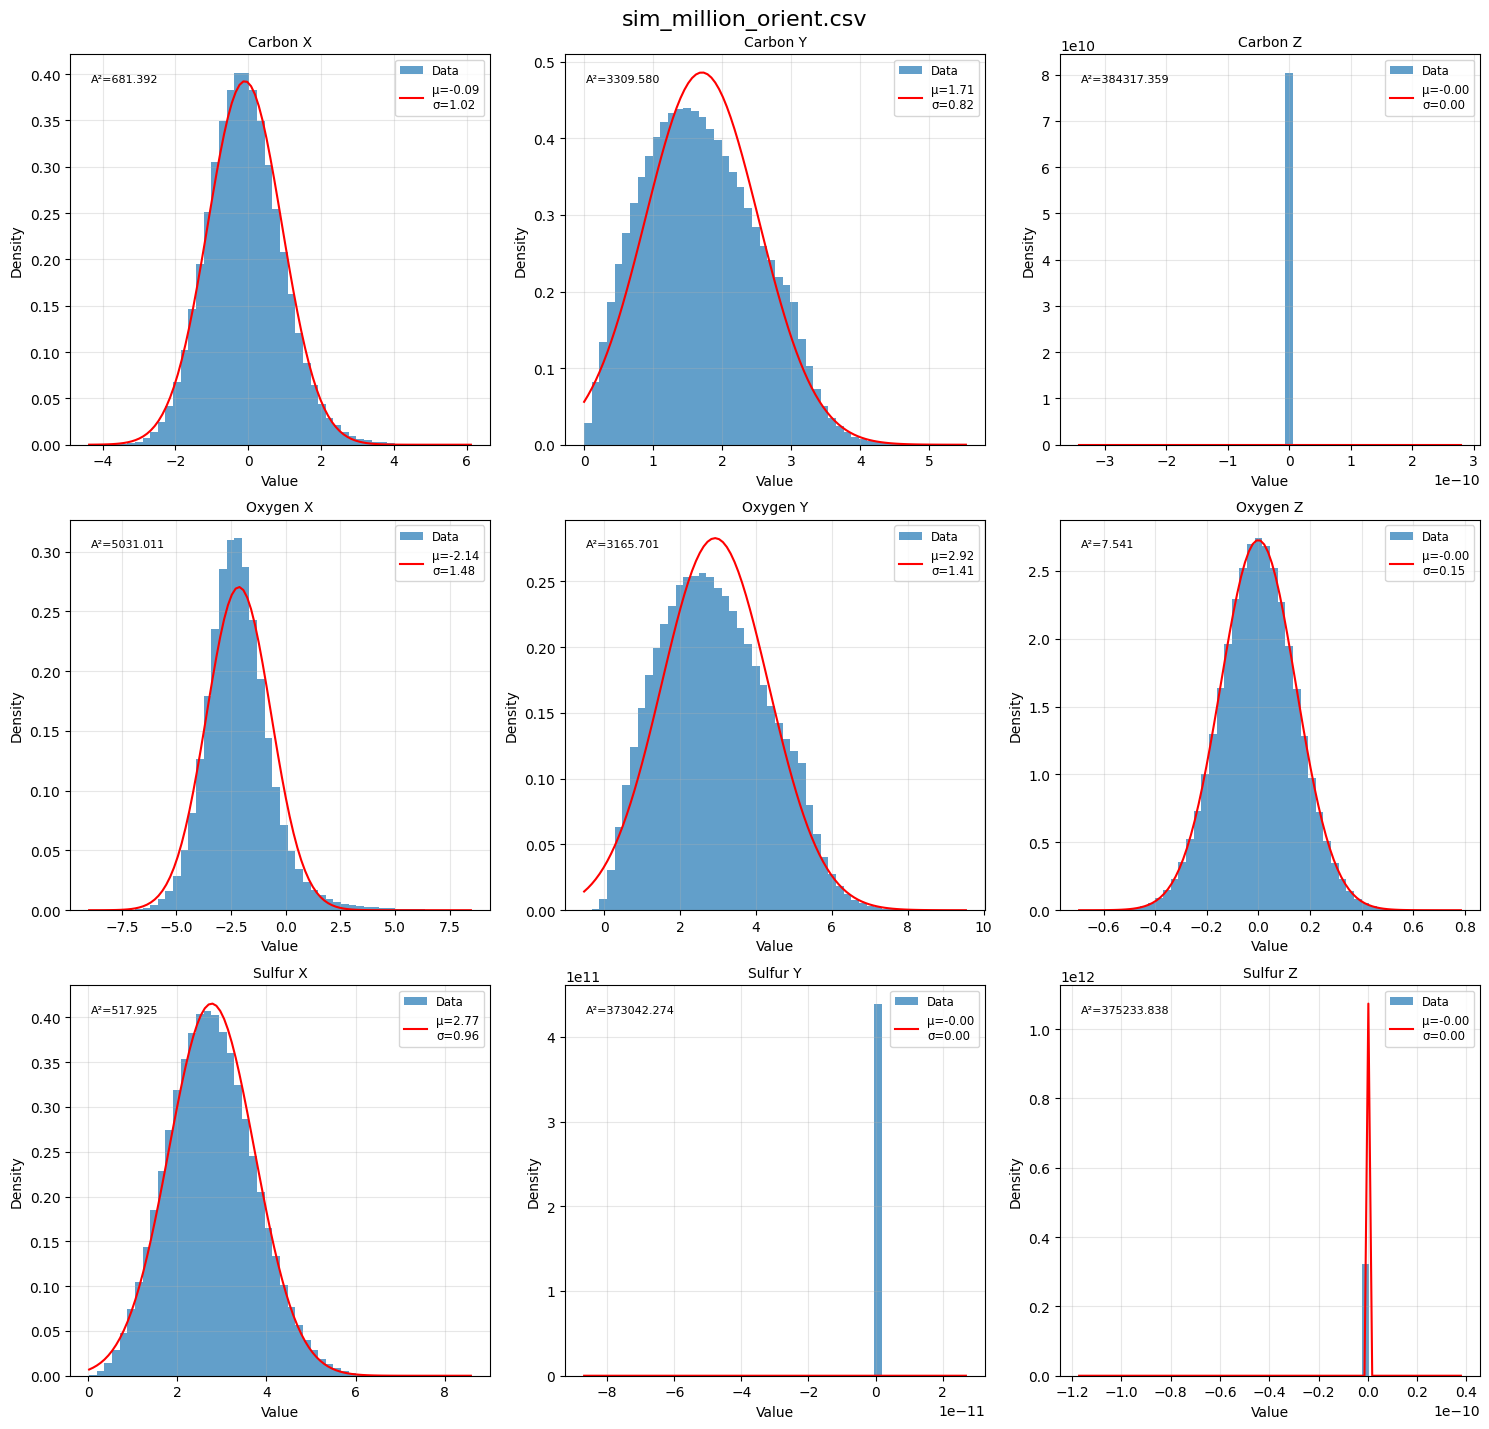
\includegraphics[width=0.6\textwidth]{sim-stats.png}
  \end{center}
\end{frame}

\begin{frame}{Test Set Prediction Plot}
  \begin{center}
    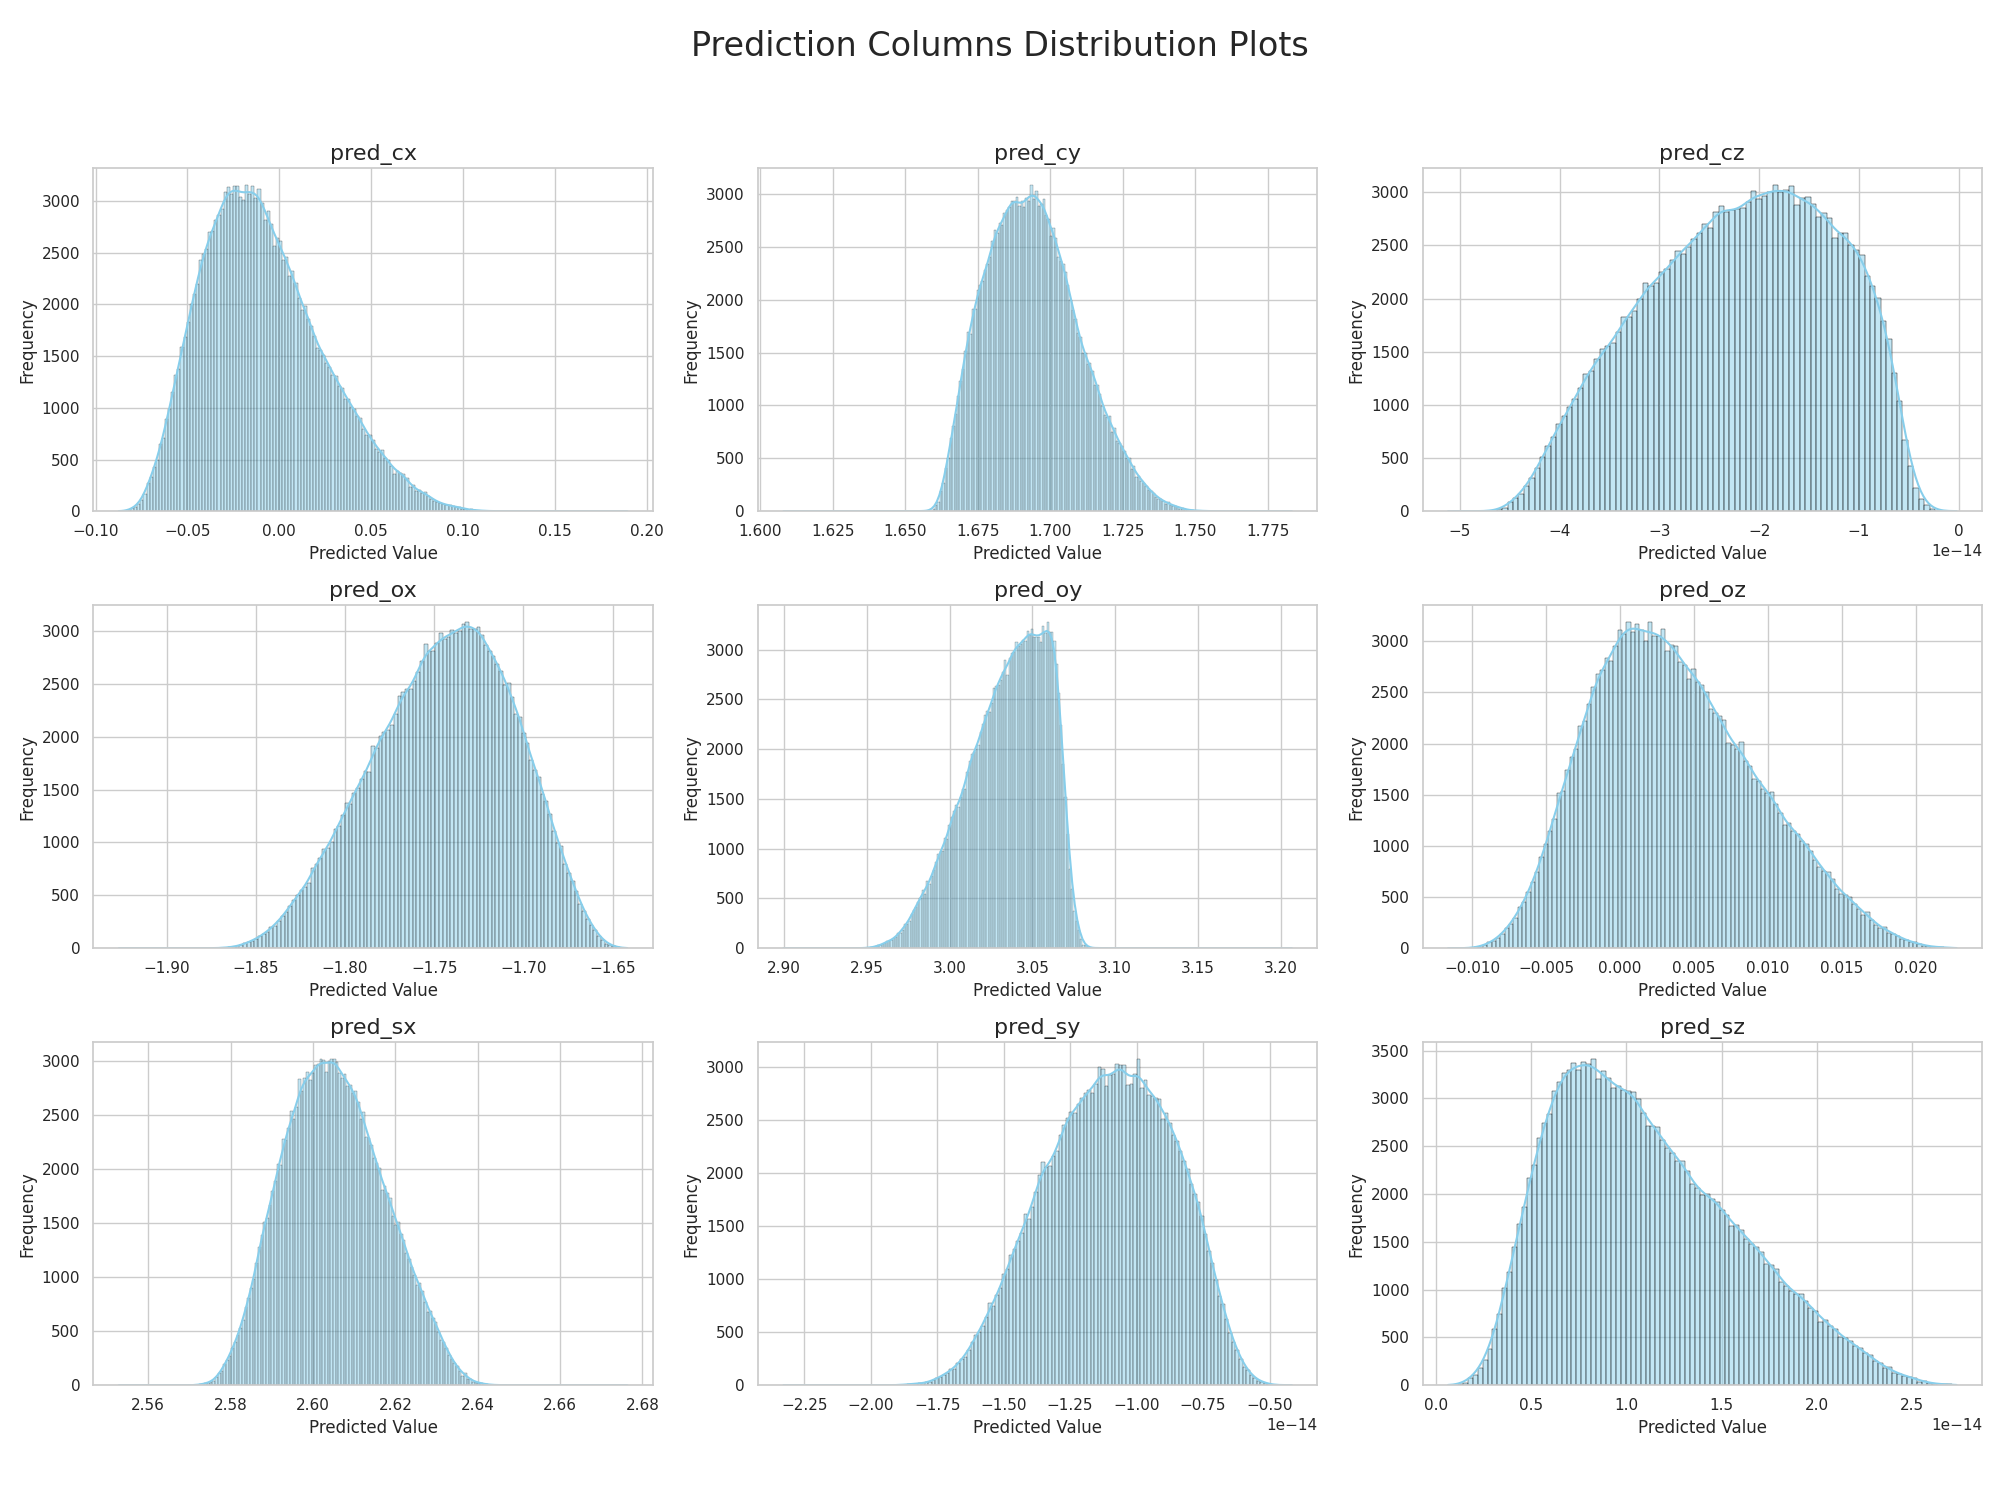
\includegraphics[width=0.9\textwidth]{predictions_distribution_plots.png}
  \end{center}
\end{frame}

% Slide 17
\begin{frame}{Performance Comparison}
  \begin{block}{Model Performance Metrics}
  \begin{center}
  \begin{tabular}{lccc}
  \toprule
  \textbf{Model} & \textbf{MRE (\%)} & \textbf{Energy Loss} & \textbf{MSE} \\
  \midrule
  \textbf{Random}        & 85.38 & $3.24 \times 10^{-1}$ & 0.17 \\
  \textbf{Sim}           & 82.67 & $4.73 \times 10^{-1}$ & 0.78  \\
  \bottomrule
  \end{tabular}
  \end{center}
  \end{block}
\end{frame}

% Slide 18
\begin{frame}{Fine-Tuning Steps, Future steps}
  Sequential steps taken to fine-tune the model:
  \begin{enumerate}
    \item \textbf{Adjusted Loss Function Weights}:
    \begin{itemize}
      \item Fine-tuned the weighting coefficients \( \alpha_1, \alpha_2, \dots, \alpha_6 \).
    \end{itemize}
    \item \textbf{Optimized Training Hyperparameters}:
    \begin{itemize}
      \item Tweaked batch size, learning rate, and increased epochs.
      \item Removed early stopping to allow full training cycles.
    \end{itemize}
    \item \textbf{Refined Regularization Factors}:
    \begin{itemize}
      \item Adjusted L1, L2 regularization strengths, and Beta.
    \end{itemize}
    \item \textbf{Enhanced Early Stopping Parameters}:
    \begin{itemize}
      \item Modified patience and \texttt{min\_delta} for better convergence.
    \end{itemize}
    \item \textbf{Explored Model Architecture}:
    \begin{itemize}
      \item Tested different configurations of layers and dimensions.
    \end{itemize}
  \end{enumerate}
\end{frame}

\end{document}
